% !TEX root = ../thesis.tex

\chapter{Motivation}
\label{cha:eva_motivation}
The most common method to reach degeneracy in a gas of ultracold atoms is by using evaporative cooling. Evaporative cooling works by selectively removing atoms from the trapped gas that are \enquote{hot} compared to the rest of the sample. The remaining atoms then equilibriate and the new equilibrium temperature is lower. This is commonly also described as cutting off the tail of the Maxwell-Boltzmann distribution. In many experiments, evaporative cooling is done in a magnetic trap, where an RF signal can be used to selectively pump atoms into an untrapped state and therefore expel them from the trap \cite{PhysRevLett.74.3352}. However, magnetic traps have the disadvantage that magnetic offset fields cannot be used as easily, for example to tune the scattering length using a Feshbach resonance \cite{PhysRevA.71.011602}. Evaporation can also be done in an optical dipole trap by lowering the laser intensity \cite{Chaudhuri_2007}. The disadvantage of optical evaporation compared to magnetic evaporation is that lowering the laser intensity is intrinsically coupled to a decrease in confinement strength for the optical trap \cite{PhysRevA.79.061406}. This leads to a reduction in density and hence increased thermalisation times, resulting in less efficient evaporative cooling.

We are interested in Bose gases with uniform density distributions. To achieve this, a box potential is necessary. However, evaporative cooling in a stationary box potential is generally unfavourable as will be shown later. Therefore, evaporation is usually carried out in a different trap first and the atomic cloud is then transferred to a box potential. Transferring the cloud is accompanied with heating and atom loss \cite{PhysRevLett.110.200406}. Our proposed solution is shown in Figure~\ref{fig:evap_box_sketch}. The cloud is trapped in a box potential immediately after a MOT and a first sub-doppler cooling stage (possibly gray molasses cooling \cite{Rosi2018enhancedGM}). Forced evaporation is then carried out by lowering the trap depth as usual. Simultaneously, the box is compressed to dynamically control the density and therefore the elastic collision rate. This would give us the opportunity to avoid one transfer step, which would help us to reduce the cycle time of the experiment. 
\begin{figure}[htbp]
    \centering
    \usetikzlibrary{arrows,positioning}
\tikzset{atom/.style={circle,draw,fill,color={rgb:red,74;blue,14;green,14},fill opacity=0.4,inner sep=0,minimum size=4pt,line width=1pt, draw opacity=0.75}}
\begin{tikzpicture}
    \node[anchor=south west] (image) at (0,0) {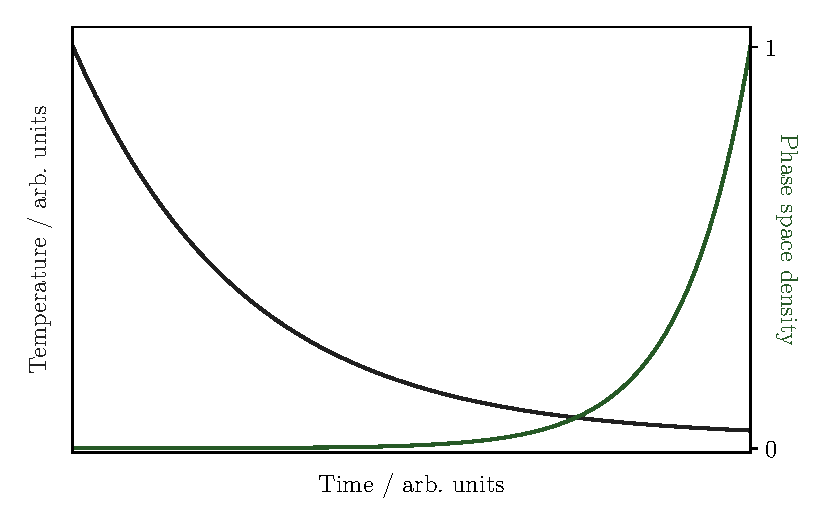
\includegraphics{Evap/BoxTrapEvaporation/baseplot}};
    \begin{scope}[x={(image.south east)},y={(image.north west)}]
        \node[anchor=north west] (large) at (0.1,0.95) {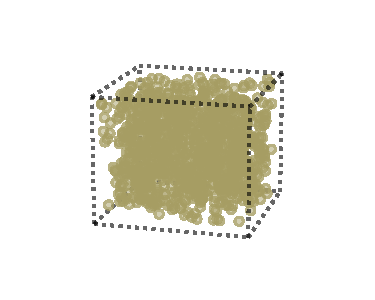
\includegraphics{Evap/BoxTrapEvaporation/Large}};
        \node[anchor=north east] (small) at (0.97,0.95) {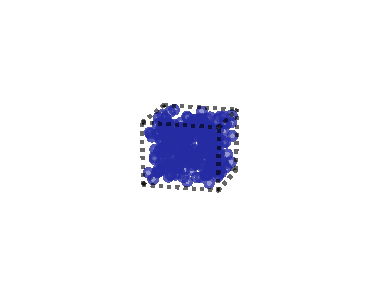
\includegraphics{Evap/BoxTrapEvaporation/Small}};
        \draw[-latex] (0.24,0.79) arc (30:110:1cm) node[below left=0.02cm and 0.13cm,atom] (A){};
        \draw[-latex] (0.44,0.8) arc (150:70:1cm) node[below right=0.015cm and 0.13cm,atom] (B){};
        \draw[-latex] (0.44,0.57) arc (70:-10:1cm) node[below right=0.134cm and -0.1cm,atom] (C){};
        \draw[-latex,thick] (0.5,0.66) -- (0.63,0.66);
    \end{scope}
\end{tikzpicture}
    \caption{Evaporative cooling in a compressing box potential}
    \label{fig:evap_box_sketch}
\end{figure}
%
In order to probe the feasability of such a system without having to build an entire experimental setup, a numerical simulation is performed. The following chapters describe the process of programming this simulation and show how this concept compares to traditional evaporative cooling processes.